\documentclass[xcolor=dvipsnames,handout]{beamer}
\usepackage{tabls}
\usepackage{graphicx}
%\usepackage{animate}
\usepackage{xcolor}

%tikz stuff
\usepackage{tikz}
\usetikzlibrary{shapes.geometric, arrows}
\tikzstyle{startstop} = [rectangle, rounded corners, minimum width=2cm, text
    width=1.5cm, minimum height=1cm,text centered, text=white,draw=black, fill=Gray!140]
\tikzstyle{io} = [trapezium, trapezium left angle=70, trapezium right angle=110,
minimum width=0.5cm, minimum height=1cm, text centered, draw=black,
fill=blue!20!Gray!90!,text=white]
\tikzstyle{process} = [rectangle, minimum width=2cm, minimum height=1cm, text
centered, text width=2cm, draw=black, text=white,fill=Gray!140!blue!70!white]
\tikzstyle{decision} = [diamond, minimum width=3cm, minimum height=1cm, text
centered, draw=black, fill=Gray!,text=white]
\tikzstyle{arrow} = [thick,line width=0.6mm,->,>=stealth]
\tikzstyle{arrow1} = [dashed,->,>=stealth]



%\definecolor{myblue}{rgb}{0.7, 0.7, 60.0}
\definecolor{mylightblue}{rgb}{1,1,1}
\newcommand*{\boxedcolor}{blue}
\makeatletter
\renewcommand{\boxed}[1]{\textcolor{\boxedcolor}{%
  \fbox{\normalcolor\m@th$\displaystyle#1$}}}
\makeatother

\renewcommand{\u}[1]{\underline{#1}}

\newcommand{\iso}[2]{${}^{{#2}}${#1} }
\newcommand{\nubar}[0]{$\overline{\nu}$ }
\newcommand{\keff}[0]{\ensuremath{{k}_{\textsf{eff}}} }
\newcommand{\expect}[1]{E[#1] }
\newcommand{\colg}[1]{{\color{ForestGreen} #1}}
\newcommand{\coly}[1]{{\color{yellow} #1}}
\newcommand{\colb}[1]{{\color{blue} #1}}
\newcommand{\colr}[1]{{\color{red} #1}}
\usepackage{amsfonts}
\newlength{\wideitemsep}
\setlength{\wideitemsep}{8pt}
%\addtolength{\wideitemsep}{5pt}
\let\olditem\item
\renewcommand{\item}{\setlength{\itemsep}{\wideitemsep}\olditem}

\newcommand{\N}{\mathbb{N}}
\newcommand{\Z}{\mathbb{Z}}
\newcommand{\deriv}[2]{\frac{\mathrm{d} #1}{\mathrm{d} #2}}
\newcommand{\pderiv}[2]{\frac{\partial #1}{\partial #2}}
\newcommand{\bx}{\mathbf{X}}
\newcommand{\ba}{\mathbf{A}}
\newcommand{\by}{\mathbf{Y}}
\newcommand{\bj}{\mathbf{J}}
\newcommand{\bs}{\mathbf{s}}
\newcommand{\B}[1]{\ensuremath{\mathbf{#1}}}
\newcommand{\Dt}{\Delta t}
\renewcommand{\d}{\mathsf{d}}
\newcommand{\mom}[1]{\langle #1 \rangle}
\newcommand{\xl}{{x_{i-1/2}}}
\newcommand{\xr}{{x_{i+1/2}}}
\newcommand{\il}{{i-1/2}}
\newcommand{\ir}{{i+1/2}}

\AtBeginSection[]
{
    \begin{frame}<beamer>
        \frametitle{Outline}
        \tableofcontents[currentsection]
    \end{frame}
}

\setbeamerfont{frametitle}{size=\large}
\setbeamerfont{normal font}{size=\tiny}

\graphicspath{{figures/}}

\usepackage{verbatim}
\usepackage{comment}
\usepackage[]{datetime}
\usepackage{multirow}

\newcommand{\thedate}{\today}


\setlength{\tabcolsep}{1.05cm}

%Aggie-themed
\pgfdeclareimage[height=0.1in]{TAMUlogo}{tamu_engineering.png}
\logo{\raisebox{-8pt}{\pgfuseimage{TAMUlogo}}}
\titlegraphic{\centering\begin{tabular}{lr}
\includegraphics[trip=4.0in 0.0in 0.0in 0.0in,clip,height=0.18\textheight]{NEUP.jpg} &

\includegraphics[height=0.18\textheight]{tamu_seal.png}\end{tabular}}
%Michigan-themed
%\pgfdeclareimage[height=0.1in]{UMlogo}{michigan_engineering.png}
%\logo{\raisebox{-8pt}{\pgfuseimage{UMlogo}}}
%\titlegraphic{
\includegraphics[height=0.2\textheight]{michigan_block_m.png}}


%%%%%%%%%%%%%%%%%%%%%%%%%%%%%%%%%%%%%%%%%%%%%%%%%%%%%%%%%%%%%%%
% Optional packages, used to show off certain tricks

\newlength \figwidth
\setlength \figwidth {0.5\textwidth}

\setlength{\leftmargin}{-2cm}
\setlength{\rightmargin}{-2cm}

%%%%%%%%%%%%%%%%%%%%%%%%%%%%%%%%%%%%%%%%%%%%%%%%%%%%%%%%%%%%%%%

\usepackage[english]{babel}
\usetheme{Frankfurt}

%Make it Aggie Maroon
\usecolortheme[RGB={80,0,0}]{structure}  
%Or Michigan Blue
%\usecolortheme[RGB={0,0,153}]{structure}  
%Or Michigan Maize
%\usecolortheme[RGB={255,204,0}]{structure}  

  % This will typeset only the frames (or slides) that have the given label ("current" in this case).

\title{A High-Order Low-Order Algorithm with Exponentially-Convergent Monte Carlo for
    $k$-Eigenvalue Problems}
\author{{\large Simon Bolding and Jim Morel}}
\date{11 November 2014 \\ \vspace{0.05in} {ANS Winter Meeting}}
\subject{}
%\institute{Los Alamos National Laboratory}

% \classificationlevel{SECRET/RD}
% \transmissible{}

%\reportnum{\textcolor{blue}{SAMPLE TEMPLATE ONLY \\ Contains NO Classified
%Information}}

% \dissableframenumber
\begin{document}

\begin{frame}
    \titlepage \vspace{-0.213in}
    \begin{center}
    \end{center}    
\end{frame}

\setlength{\tabcolsep}{6pt}

\begin{frame}
\frametitle{Outline}
\begin{minipage}{0.061\linewidth}
\hfill                      
\end{minipage}
\begin{minipage}{0.8\linewidth}
\tableofcontents[
hideothersubsections,
sectionstyle=show,
subsectionstyle=hide
]
\end{minipage}

\end{frame}


\section{Overview}


\begin{frame}
    \frametitle{A High-Order Low-Order Solution}
        \begin{itemize}
            \item[]<1-> \begin{block}{Basic Idea} Build a low-order (LO) system that can be efficiently solved,
                with high-order (HO) correction from pure absorber MC simulations \end{block}
                \vspace{-0.1in}
              \item Useful when global solution of particle density needed, with low
                  statistical noise
              \item<1-> The LO solution
                  preserves the HO solution, upon 
                  convergence (consistent)
              \item<2-> The LO solver handles non-linearities and inscattering source
                \begin{itemize}
                    \item<2-> Produces a linear-discontinuous (LD) representation of sources
                    \item<2-> Lower \colb{dimensional} problem
                  %  \item Consistency terms derived directly from transport equation
                \end{itemize}

            \item<3-> The HO system is a fixed-source transport problem
                \begin{itemize}
                    \item<3-> ECMC allows for the statistical noise to be reduced
                        globally, giving accurate consistency terms
                \end{itemize}
        \end{itemize}
\end{frame}


\begin{frame}
    \frametitle{The Thermal Radiative Transfer Equations}
    \begin{itemize}
        \item 1D, gray, isotropic scattering, backward Euler 
        \item $\sigma$ can be a function of $T$
        \item \colb{Transport} equation
    \begin{equation*}
\mu \pderiv{I^{n+1}}{x} + \left(\sigma_t + \frac{1}{c \Delta t }\right) I^{n+1}
= \frac{\sigma_s}{2} \phi^{n+1} +\frac{1}{2} \left(\sigma_a a c T^4
\right)^{n+1} + \frac{I^n}{\Delta_t c}  
    \end{equation*}
    \pause
    \vspace{-0.2in}
\item \colb{Material energy} equation
        \begin{equation*}
\rho c_v \frac{T^{n+1} - T^n}{\Delta t} = \int_{-1}^{1} \sigma_a I^{n+1}(x,\mu)
\d\mu - \left(\sigma_a a c T^4\right)^{n+1} 
    \end{equation*}
\begin{equation*}
    \phi(x) = \int_{-1}^1 I^{n+1}(x,\mu) \d\mu
\end{equation*}
\end{itemize}
\end{frame}

\begin{frame}
    \frametitle{Eigenvalue Problem}
    \begin{itemize}
        \item 1D transport equation
    \begin{equation*}
    \mu \pderiv{\psi}{x} + \Sigma_t \psi(x,\mu)
    = \frac{1}{4\pi}\left(\Sigma_s  + \frac{\nu \Sigma_f}{\keff} 
    \right) \phi(x)
    \end{equation*}
    \pause
    \vspace{-0.2in}
\begin{equation*}
    \phi(x) = 2 \pi \int_{-1}^1 \psi(x,\mu) \d\mu
\end{equation*}
    \item MC solutions typically use power iteration
        \begin{itemize}
            \item Accelerate source convergence with LO solution (e.g., CMFD)
        \end{itemize}
        \begin{block}{} We will use a low-order solution that handles the scattering
        and fission operators to determine $\keff$ and $\phi(x)$. The LO solution preserves MC transport solution\end{block}
\end{itemize}
\end{frame}






\section{Low-Order Solver}

\begin{frame}
    \frametitle{LO Discretization \& Space-Angle Moments}
    \begin{itemize}
        \item Linear Discontinuous (LD) finite elements in space and half range
            angular integrals
    \end{itemize}
    \begin{figure}
    \begin{centering}
        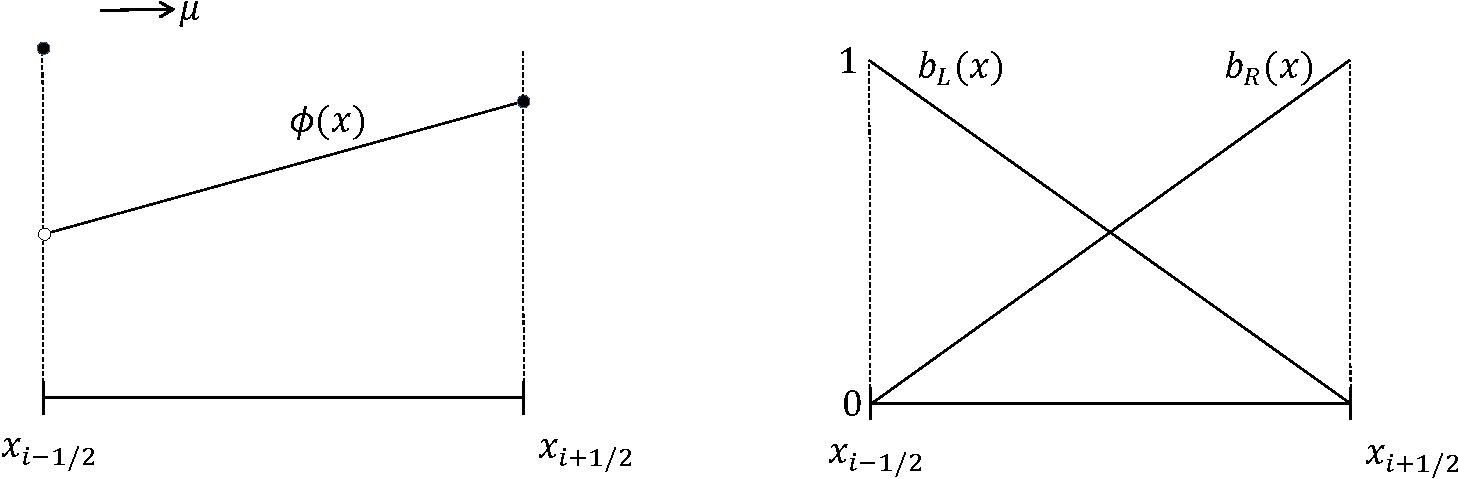
\includegraphics[width=0.9\textwidth]{LD.pdf}
    \end{centering}
    \end{figure}
    \begin{center}
    \begin{tabular}{cc}
        \underline{Spatial moments} & \underline{Angular half-ranges} \\ 
        $ {\displaystyle \mom{\cdot}_{L,i} = \frac{2}{h_i} \int_{x_\il}^{x_\ir}
        b_{L,i}(x)(\cdot) \d x \quad }$  & ${ \quad \displaystyle \phi^+(x) = 2\pi\int_0^1 I(x,\mu) \d \mu}$
    \end{tabular}
    \end{center}

\end{frame}




\begin{frame}
    \frametitle{LO System}
    \begin{itemize}
        \item Taking moments of TE yields \colb{4 equations}, per cell $i$, e.g.
        {\small
        \begin{multline*}\label{lo_tran}
    -2{\mu}_{i-1/2}^{+} \phi_{i-1/2}^{+} + \mom {\mu}_{L,i}^{+}
  \mom{\phi}_{L,i}^{+}
  +  \mom\mu_{R,i}^{+}
  \mom{\phi}_{R,i}^{+} + \\ \Sigma_t h_i \mom{\phi}_{L,i}^+ -  \frac{\Sigma_s h_i}{4\pi} \left( \mom{\phi}_{L,i}^{+} +
  \mom\phi_{L,i}^{-}\right) = \frac{1}{\keff} \frac{\nu \Sigma_fh_i}{4\pi}\mom{\phi}_{L,i}^{+}
\end{multline*}}
        \item Cell unknowns: $\mom{\phi}_{L,i}^{+}$, $\mom{\phi}_{R,i}^{+}$,
        $\mom{\phi}_{L,i}^{-}$, $\mom{\phi}_{R,i}^{-}$ 

    \item Need \colb{angular} consistency terms  and spatial closure
        (LD)
    \end{itemize}

\end{frame}


\begin{frame}
    \frametitle{Computing LO Consistency terms from HO Solution}
    \begin{itemize}
        \item For $\mu>0$, $L$ moment
    \begin{equation}
\mom{{\mu}}_{L,i}^{+} \simeq \frac{\displaystyle 
\frac{2}{h_i} \int\limits_0^1 \int\limits_\xl^\xr \mu \, b_{L,i}(x) \tilde \psi^{HO}(x,\mu) \d \mu \d x } 
{\displaystyle \frac{2}{h_i} \int\limits_0^1 \int\limits_\xl^\xr \, b_{L,i}(x)
\tilde \psi^{HO}(x,\mu) \d \mu \d x } 
    \end{equation}
        \item ECMC gives LDFE $\tilde  \psi^{HO}(x,\mu)$ for computing terms directly
        \item To get S$_2$, set $\mom{\mu}^\pm = \pm \frac{1}{\sqrt{3}}$ 
    \end{itemize}

\end{frame}

\begin{frame}
    \frametitle{Solving LO System with Power Iteration}
    \begin{itemize}
        \item Global System: \hspace{0.8in}${\displaystyle \B D \Phi = \frac{1}{\keff} \B F \Phi}$
     \end{itemize}
     \begin{block}{Algorithm}
         \begin{enumerate}
        \item Guess $\Phi^{(0)}$ and $\keff^{(0)}$
        \begin{align*}
    \Phi^{(l+1)} = \frac{1}{\keff^{(l)}} \B D^{-1} \B F \Phi^{(l)} \\
    \quad \keff^{(l+1)} = \keff^{(l)}\frac{ \int \nu \Sigma_f \phi^{(l+1)} \d
    x}{ \int \nu \Sigma_f \phi^{(l)}\d x }.
        \end{align*}
    \item Converge $\phi(x)$ and \keff \pause
    \item \colb{Accelerate} $\Phi^{(l)}$ and $\keff^{(l+1)}$ after each power iteration
        with Nonlinear Krylov Acceleration (NKA)
     \end{enumerate}
    \end{block}
\end{frame}

\section{High-Order Solver}

\begin{frame}
    \frametitle{Exponentially Convergent Monte Carlo}
    \begin{itemize}
        \item An iterative form of residual Monte Carlo
        \item Requires a functional form of the angular flux in space and angle
            \begin{itemize}
                \item Use finite element representation
            \end{itemize}
    \item Can reduce statistical error \colb{globally} $\propto e^{-\alpha N}$
            \begin{itemize}
                \item Does not make difficult problems easier
            \end{itemize}
        \item Adaptive mesh refinement allows the error to continue to be reduced
            \begin{itemize}
                \item Increase $N$ per batch by factor of new cells added
            \end{itemize}
    \end{itemize}


\end{frame}

\begin{frame}
    \frametitle{Space-Angle Mesh and MC Implementation Details}
    \noindent
    \begin{minipage}[t]{0.36\linewidth}
        \centering
        \scalebox{0.8}{
        \begin{tikzpicture}
            \draw (1,1) rectangle (4,4);
            \node[draw,circle,inner sep=1.2 pt,fill] at (2.5,2.5) {};
            \node[above] at (2.5,2.5) {$(x_i,\mu_j)$};
            \draw (1.0,0.4) -- (1.0,0.6) node[below, pos=0.4] {$x_{i-1/2}$};
            \draw (4.0,0.4) -- (4.0,0.6) node[below, pos=0.4] {$x_{i+1/2}$};
            \draw (0.4,1.0) -- (0.6,1.0) node[left, pos=0.4] {$\mu_{j-1/2}$};
            \draw (0.4,4.0) -- (0.6,4.0) node[left, pos=0.4] {$\mu_{j+1/2}$};
            \draw [thick,->] (0.5,0.5) -- (5,0.5) node[anchor=north west] {$x$};
            \draw [thick,->] (0.5,0.5) -- (0.5,5) node[anchor=east] {$\mu$};
        \end{tikzpicture}
    }
    \end{minipage}%
    \begin{minipage}[t]{0.70\linewidth}
        \vspace{-1.6in}
        \begin{itemize}
            \item {\small $\displaystyle \tilde \psi(x,\mu) = \psi_{a,i} + \psi_{x,i}
                \frac{2}{h_{x}}(x-x_i) + \psi_{\mu,i}
            \frac{2}{h_{\mu}}(\mu-\mu_i)$}
        \item Path-length estimators of moments, e.g.
            {\small
            \begin{align*}
                \psi_{x,i} &= \frac{6}{h_{x}^2h_\mu}
             \iint\limits_\mathcal{D} (x_{c,j}-x_i) \psi(x,mu) \d x \d \mu 
        \end{align*}}    
        \end{itemize}
    \end{minipage}
    \begin{itemize}
        \item Particles are allowed to stream, $w(s)=w_0 e^{-\Sigma_t s}$
        \item LDFE and upwinding \colb{eliminates} surface tallies
    \item Cell-wise, global representation allows for \colb{stratified} sampling
        \begin{itemize}
            \item $N_{i,j} \propto{|r_i(x,\mu)|}$
            \item Force $N_i \geq N_{\min}$ and adjust particle weights
        \end{itemize}

    \end{itemize}

\end{frame}


\begin{frame}
    \frametitle{High Order System and ECMC Algorithm}
    \begin{itemize}
        \item \colb{Pure absorber} transport problem
        \begin{align*}
            \left[\mu \pderiv{}{x} + \Sigma_t\right]\psi(x,\mu)
            &= \boxed{\frac{1}{4\pi}\left(\Sigma_s + \frac{1}{\keff^{LO}}\right)
        \phi^{LO}(x)} \\
         \B L \psi &= q^{LO}
     \end{align*}
        \vspace{-0.3in}
        \end{itemize}
        \begin{block}{ECMC Algorithm}
         \begin{itemize}
        \item Residual Equation: $\displaystyle \B L \tilde 
            \epsilon^{(m)} =
            \tilde r^{(m)} = q^{LO} - \B L \tilde\psi^{(m)}$
            \vspace{0.01in}
        \item Compute $\tilde{\epsilon}^{(m)} = \B L^{-1} \tilde{r}^{(m)}$ with MC,
            \colb{projecting} the solution  
        \item Update: $\tilde\psi^{(m)} = \tilde\psi^{(m-1)} + \tilde \epsilon^{(m)}$
        \begin{itemize}
            \item If $\tilde{\epsilon}$ is reduced each batch, \colb{exponential convergence
                achieved}
            \item $h$-refine when $\epsilon(x,\mu)$ not represented sufficiently
             \item Must sufficiently reduce noise in $\epsilon$ tallies, each batch
        \end{itemize}
    \item Repeat until $\| \tilde \epsilon \|_2 < \textsf{tol}\times \| \psi \|_2$
    \end{itemize}
\end{block}

\end{frame}

\section{High-Order Low-Order Algorithm}

\begin{frame}
    \frametitle{High-Order Low-Order Algorithm}
    %\fontsize{9}{5.0}\selectfont
    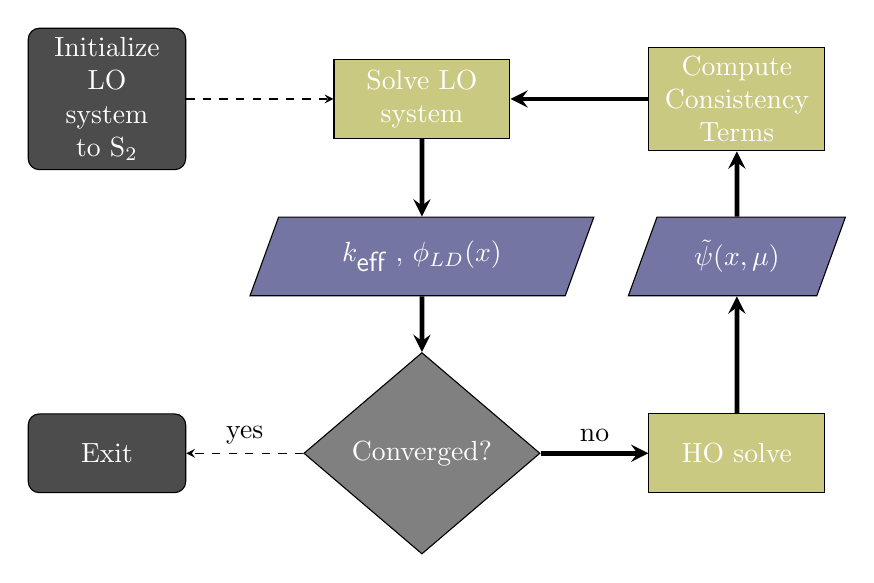
\begin{tikzpicture}[node distance=2cm]
        \node (start) [startstop] {Initialize LO system to S$_2$};
        \node (in1) [process, right of=start, xshift=2cm] {Solve LO system};
        \node (pro1) [io, below of=in1] {\keff, $\phi_{LD}(x)$};
        \node (dec1) [decision, below of=pro1, yshift=-0.5cm] {Converged?};
        \node (pro2a) [startstop, left of=dec1, xshift=-2.0cm] {Exit};
        \node (pro2b) [process, right of=dec1, xshift=2cm] {HO solve};
        \node (out1) [io, above of =pro2b, yshift=0.5cm] {$\tilde{\psi}(x,\mu)$};
        \node (cons) [process, above of=out1] {Compute Consistency Terms};
        

        \draw [arrow1] (start) -- (in1);
        \draw [arrow] (in1) -- (pro1);
        \draw [arrow] (pro1) -- (dec1);
        \draw [arrow] (dec1) -- node[anchor=south] {no} (pro2b);
        \draw [arrow1] (dec1.west) -- node[anchor=south] {yes} (pro2a);
        \draw [arrow] (pro2b) -- (out1);
        \draw [arrow] (cons) -- (in1);
        \draw [arrow] (out1) -- (cons);
    \end{tikzpicture}
\end{frame}

\section{Results}
\begin{frame}
    \frametitle{\coly{Critical slab benchmark}}
    \fontsize{9}{5.0}\selectfont
    \begin{block}{Problem Parameters}
    \begin{itemize}
        \item $k_\infty = 2.29$, $\Sigma_t = 0.326$ cm$^{-1}$
        \item 2.4$\times10^5$ histories per batch, 100 $x$ \& 20 $\mu$ cells
        \item Adaptive HO convergence
    \end{itemize}
    \end{block}
    \begin{minipage}{0.49\textwidth}
    \begin{figure}
    \centering
    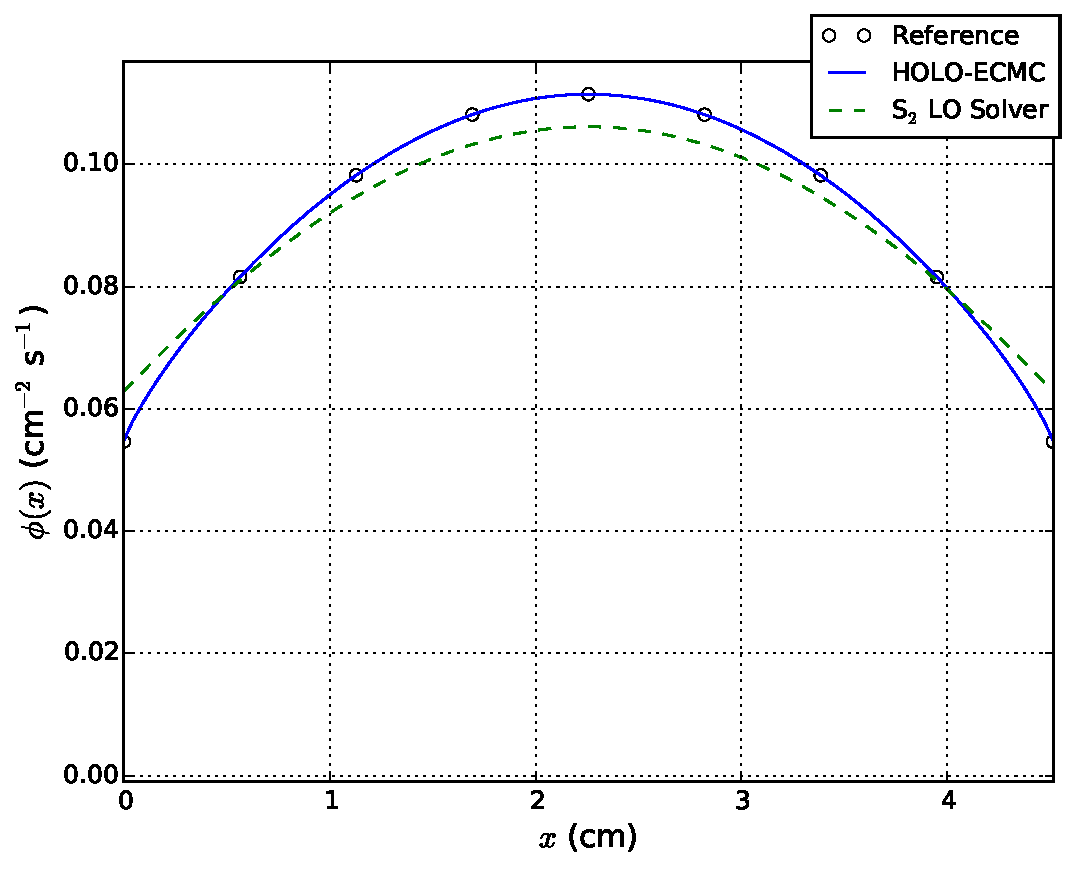
\includegraphics[width=0.98\textwidth]{sood_fiss_src.pdf}
    \end{figure}
    \end{minipage}
    \begin{minipage}{0.49\textwidth}
    \begin{itemize}
        \item $|\Delta \Phi| < 10^{-4}$ in 4 outer iterations, using            $\sim2.4\times10^7$ histories
        \item For 10 independent simulations:
            \begin{itemize}
                \item  $\overline{\keff} = 0.999998$,
                    $\sigma(\keff)=4.1\times10^{-6}$, max dev. $=1.1\times10^{-5}$
                \item $\overline{\sigma_{\text{rel}}(\phi_i)} = 1.4\times10^{-05}$
            \end{itemize}
    \end{itemize}
    \end{minipage}
\end{frame}

\begin{frame}
    \frametitle{\coly{Optically thick, near-critical slab}}
    \fontsize{9}{5.0}\selectfont
    \begin{block}{Problem Parameters}
    \begin{itemize}
        \item $k_\infty = 1$, $\Sigma_t = 30.0$ cm$^{-1}$, $\Sigma_s=29.5$ cm$^{-1}$,
            DR$\simeq$\textbf{0.999}
        \item Relative Tolerance of 1.0E-05 for all solvers
    \end{itemize}
    \end{block}
    \begin{minipage}{0.49\textwidth}
    \begin{figure}
    \centering
    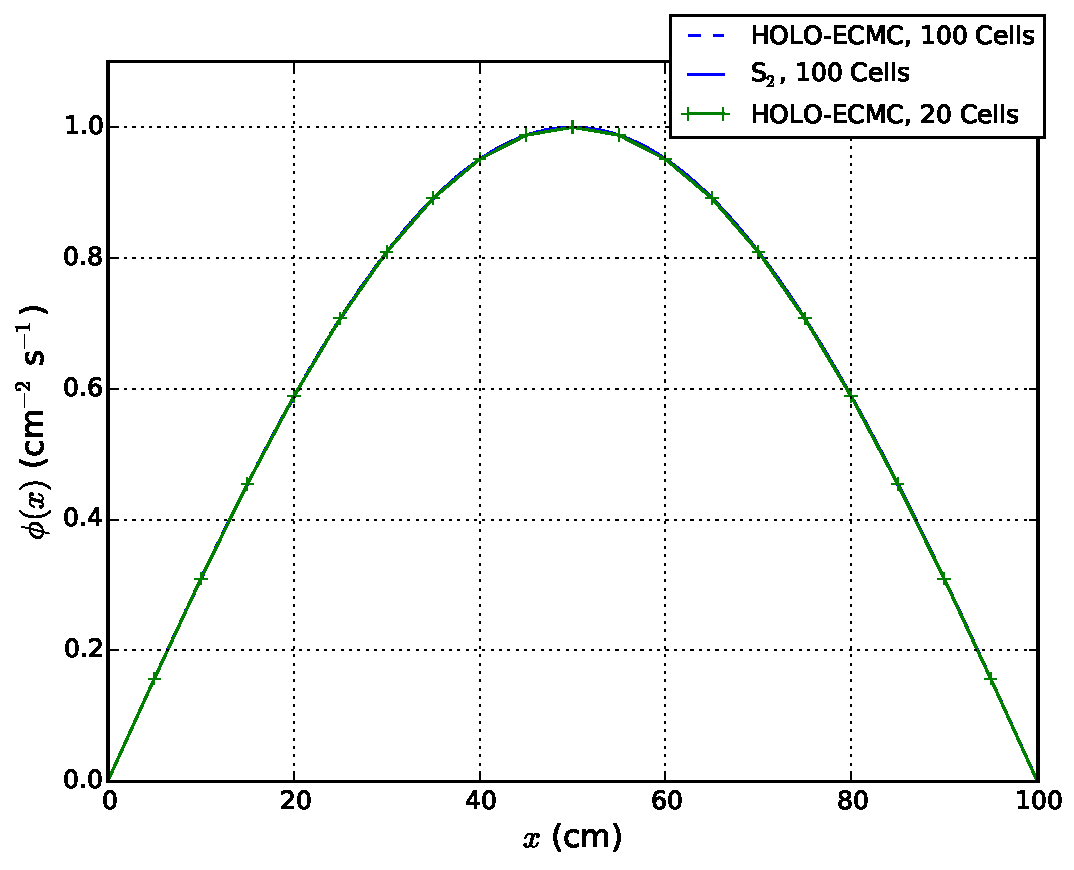
\includegraphics[width=0.98\textwidth]{highdr_fiss_src.pdf}
    \end{figure}
    \end{minipage}
    \begin{minipage}{0.49\textwidth}
        \begin{itemize}
            \item Fission source convergence:
            \begin{itemize}
            \item Power iteration not converged after 10,000 iterations
            \item NKA converged in 246 iterations
            \end{itemize}
            \item 1 outer iteration, 4.8$\times 10^6$ total histories
            \item $\keff = 0.99997$ 
        \end{itemize}
    \end{minipage}
\end{frame}

\begin{frame}
    \frametitle{Comparison of statistical noise for standard and ECMC HO solvers}
    \begin{block}{}
    \begin{itemize}
        \item One HO solve, with a fixed number of histories $N$. Comparison of
            \colr{ECMC} with 5 batches or standard MC (\colb{SMC}) 
    \end{itemize}
    \end{block}
  \begin{minipage}{0.49\textwidth}
  \begin{figure}
    \centering
    \underline{Critical Slab}
    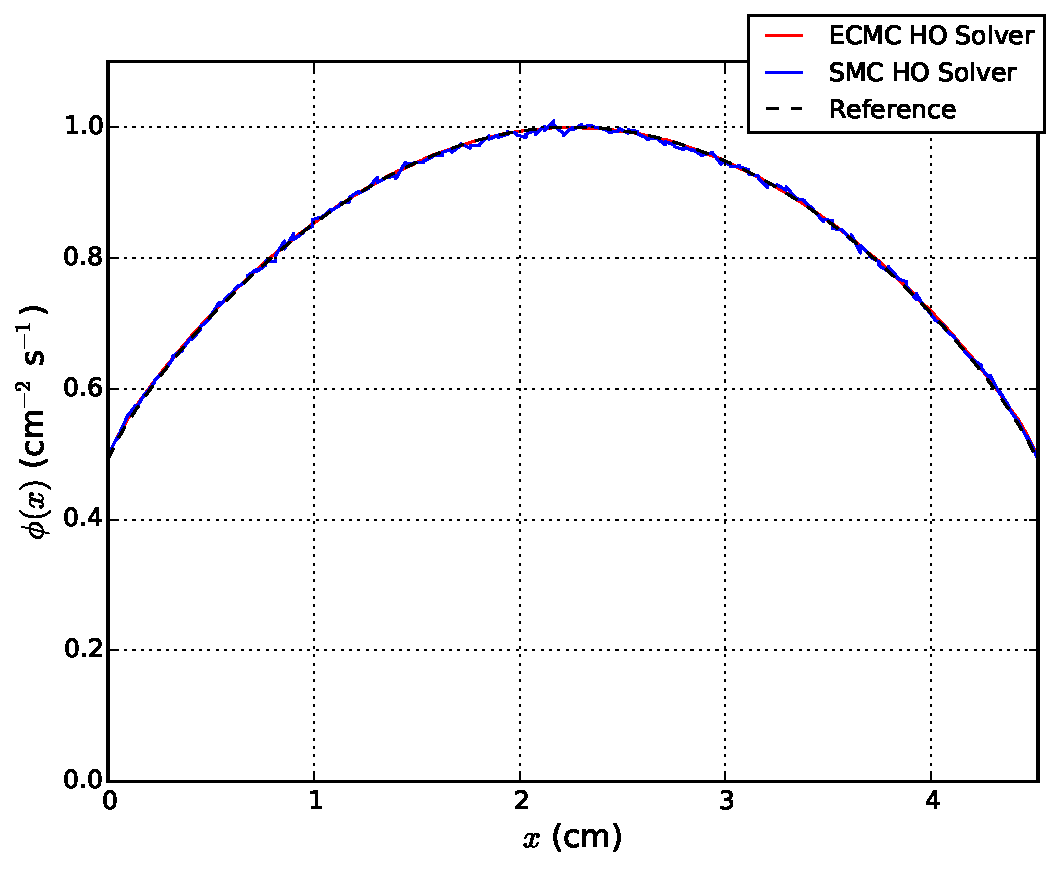
\includegraphics[width=0.89\textwidth]{sood_smc_compare.pdf} \\
      \hspace{0.1in}$N=1.5\times10^5$
  \end{figure}
  \end{minipage}
  \begin{minipage}{0.49\textwidth}
  \begin{figure}
    \centering
    \underline{Diffuse Slab, $k_\infty=1$}
    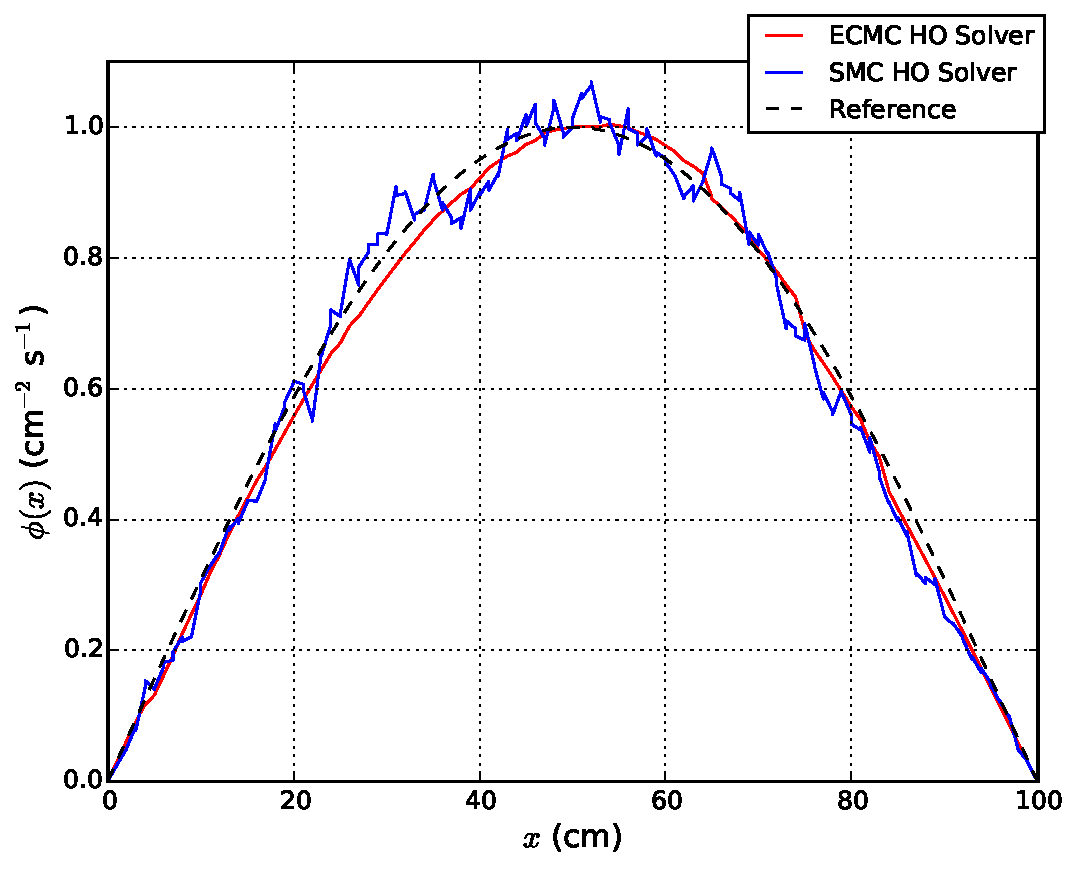
\includegraphics[width=0.89\textwidth]{smc_compare.pdf} \\
    \hspace{0.3in}$N=10^6$
  \end{figure}
  \end{minipage}

\end{frame}

\section{Conclusions}

\begin{frame}
    \frametitle{Current \& Future Development}
    \begin{itemize}
        \item Can Solve for $\keff$ and fission source with HOLO method
        \begin{itemize}
            \item Pure absorber histories are cheaper than standard MC simulations
            \item ECMC efficiently reduces noise globally 
            \item LO solver handles scattering, fission, and 
        \end{itemize}
        \item Stratified source sampling more efficient at reducing statistical
            variance than a constant number of particles per cell
        \item Need to use the estimated statistical error in tallies for $\tilde\epsilon(x,\mu)$ 
    \end{itemize}

\end{frame}


\date{11 November 2014}

\begin{frame}
    \frametitle{{\LARGE\coly{Questions?}}}
    \titlepage \vspace{-0.113in}
\end{frame}

\appendix

\title{Backup Slides}
\author{}
\date{}

\begin{frame}
    \titlepage
\end{frame}


\begin{frame}
    \frametitle{ECMC procedure}
    {
    \begin{block}{Algorithm}
    \begin{enumerate}
        \item $\tilde \psi^{(0)}=\tilde \psi$ or from last batch this time step
        \item Using Monte Carlo, solve $\epsilon^{(m)} = \B L^{-1} \tilde r^{(m)}$
            \begin{itemize}
                \item Use volumetric tallies, weighted with $x$ and $\mu$ basis moments time $\psi$ to construct LD
                    $\tilde\epsilon^{(m)}(x,\mu)$ over the current space-angle mesh
            \end{itemize}
        \item $\tilde \psi^{(j+1)} = \tilde \psi^{(m)} + \tilde \epsilon^{(m)}$
        \item \textbf{IF} error stagnation:
            \begin{itemize}
                \item Refine mesh based on relative jump error in $\tilde \psi(x,\mu)$
            \end{itemize}
        \item Repeat 2-4 until $\| \tilde \epsilon \|_2 < \textsf{tol}\times
            \|\psi\|_2$
    \end{enumerate}
    \end{block}
}
\end{frame}

\begin{frame}
    \frametitle{HOLO Algorithm}
    {
    \begin{block}{Algorithm}
        \begin{enumerate}
            \item Initialize $\mom{\mu}^{\pm}$ parameters to S$_2$
            \item Solve LO system using power iteration
            \item Build $q^{LD}$ for HO solver, and set $\tilde{\psi}$ to latest
                HO estimate
                on coarsest $x$--$\mu$ mesh
            \item Solve $\tilde \psi(x,\mu) = \B L^{-1}q^{LO}$ using ECMC
            \item Compute new $\mom{\mu}^\pm$ parameters using $\tilde \psi^{HO}$ over LO mesh
            \item Repeat 2-5 until $\underline \Phi^{LO}$ is converged
        \end{enumerate}

    \begin{itemize}
        \item Use adaptive convergence criteria
    \end{itemize}
    \end{block}
}
\end{frame}

\begin{frame}
    \frametitle{Exponential Convergence Plot}






\end{frame}

\end{document}
